% !TEX root = ../master-thesis.tex

\begin{figure}
    \centering
    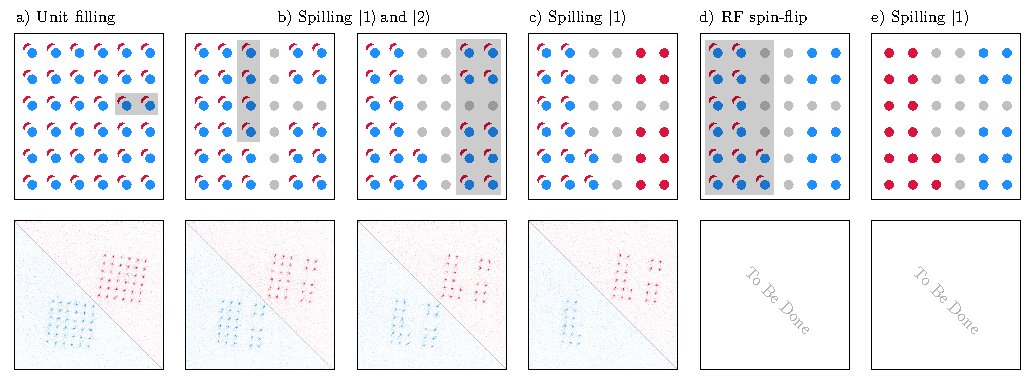
\includegraphics{fig-ai/preparation-array-ai.pdf}
    \caption{
    \textbf{Sequence for arbitrary filling preparation in a 2D tweezer array.}
    \textit{Top row}: Schematics of spin- and site-selective atom spilling, with gray shading indicating regions where atoms are removed. Blue and red semicircles represent atoms in different spin states, while gray circles denote emptied sites.
    \textit{Bottom row}: Experimental snapshots (averaged over 10 realizations) demonstrating each preparation stage. Panels (a)-(c) show completed experimental steps: initial unit filling (a), spilling of both spin states from selected regions (b), and spin-selective spilling of state $\ket{1}$ atoms (c). Panels (d)-(e) illustrate future planned steps, including spin-flip via RF transition (d) and subsequent spilling (e), which have not yet been experimentally realized.
    % due to pending hardware installation
    }
    \label{fig:preparation-array}
\end{figure}




After balancing the tweezer depths and performing standard spilling to prepare unit filling (one atom in state $\ket{1}$ and one in $\ket{2}$ per site), atoms in a selected spin state can be selectively removed while leaving the other unaffected. This enables the preparation of arbitrary spin-resolved configurations, a crucial ingredient for bottom-up simulation of spinful many-body systems.

% \textbf{Magnetic-field dependence.}
The key idea relies on the difference in magnetic moments between the hyperfine ground states. As shown in Fig.~\ref{fig:li6levels}b, the energy of state $\ket{2}$ exhibits a maximum near $27\,\mathrm{G}$, where its magnetic moment vanishes: $\mu_{|2\rangle} = \partial E / \partial B = 0$. In contrast, state $\ket{1}$ has a sizable negative magnetic moment at this field.
% \red{(write down value)}. 
As a result, when a magnetic field gradient is applied at $B = 27\,\mathrm{G}$, only atoms in state $\ket{1}$ experience a significant force and are spilled from the traps.

% \textbf{Spin-selective removal.}
The experiment starts with a $\ket{1}$–$\ket{2}$ spin mixture at unit filling in each tweezer. The magnetic field is ramped to $27\,\mathrm{G}$, and a field gradient is applied. This results in spin-selective spilling: atoms in state $\ket{1}$ are removed, while those in $\ket{2}$ remain confined.

The crossed AOD configuration enables control over the local optical power $P_{ij}$ through factorized amplitudes, such that $P_{ij} = H_i V_j$. This allows us to define arbitrary rank-1 intensity masks and thus selectively apply spilling to specific subsets of sites. 
% In this way, we can prepare structured spin patterns such as stripes, checkerboards, or arbitrary factorized configurations.
This protocol enables single-shot removal of state $\ket{1}$ atoms without perturbing state $\ket{2}$, providing a flexible method for initializing spin-imbalanced or spatially patterned states. 
% The performance of the method in terms of selectivity and overall fidelity is summarized in \red{Fig.~?}. 
Sequential applications of such steps to prepare arbitrary configurations are discussed in Sec.~\ref{subsec:arbitrary-occupation-loading}.
